\subsection*{Stop, Question, and Frisk data}

The legal sector is one in which ADMs have been deployed, more often than not accompanied by public debate and protests about targeted policing and racial discrimination (COMPASS as the most popular example). We will turn our focus to the stop, question, and frisk (SQF) dataset published by the New York police department (NYPD). A. Fabris and S. Messina and G. Silvello and G.A. Susto scanned more than x datasets to diversify the datasets that are used in the fairness literature. They recommend it as suitable dataset for fairness research. First, we will give some context to the dataset. We will continue with descriptive analysis and finally examine fairness of an algorithm trained on this data.

Since x the stop, question, and frisk practice is implemented in New York City. A police officer is allowed to stop a person if they have reasonable suspicion that the person has committed, is committing, or is about to commit a crime.
During the stop the officer is allowed to frisk a person (pat-down the person's outer clothing) or search them more carefully.
The stop can result in a summon, an arrest or no further consequences. After a stop was made, the officer is required to fill out a form, documenting the stop. This data is published yearly by the NYPD.
Many citizens have critisised the stop and frisk practice. There is disagreement about whether the strategy is effective in reducing the crime rates of the city {\color{red}cite some studies}. The police has been repeatedly critisised for over-targetting people of colour.
Stop and Frisk practice during 2004 to 2012 has been deemed as unconstitutional. {\color{red} source}

\subsubsection*{Data description}
For our analysis we look at the stops from 2023 as they were the most recent recordings at the time of writing this paper. The raw 2023 dataset consists of 16971 observations and 82 variables. We first discarded all the variables that have more than 20\% missing values.
34 variables remain that provide us with information about the stop and demographic information of the stopped person. From this reduced dataset we filter out the complete cases and end up with 12039 observations.
\footnote{Simply discarding the missing values and only training on complete cases is discouraged by \cite{fernando2021}. We opt for this approach regardless, since imputation of the missing values is not straight forward
but treating missing values as an extra category (which some random forest learners in mlr3 can do) will introduce complications when we implement some fairness methods later on.}
% (many fairness methods can not deal with missing data, especially in the protected attribute, which makes sense, since they base their decision on it). 
We choose the arrestment of a suspect as target and the race as protected attribute. For the fairness audit later in the chapter we dichtotomise the PA to adjust our situation to the common binary classification, binary PA scenario in the fairness literature. For the descriptive analysis we leave align the race description of SQF data with the 2021 census data. Thereby placing "Black Hispanic" into the group "Black" and summarising "American Indian/ Native American" of SQF and "Middle Eastern/ Southwest Asian" of SQF into the "Other" category.  
In the cleaned 2023 data about 31\% of stops result in an arrest. Overall racial disparities in arrestment rates are low. The arrestment rate for white suspects is the highest. \autoref{fig:arrestment_rates_clean_data}. As group fairness metrics are observational and constructed from the joint probability of $Y, \hat{Y}, A$ alone, this already gives us a hint that the classifier will show little racial disparities.
% \footnote{This, of course, is an oversimplification of the scenario and we know that this grouping can be critisised from a social science standpoint. We see this as a compromise to keep things straight forward. More nuanced scenarios can be addressed in future work.} 


\subsubsection*{Fairness Auditing}
% insert a graphic
\begin{figure}
    \centering
    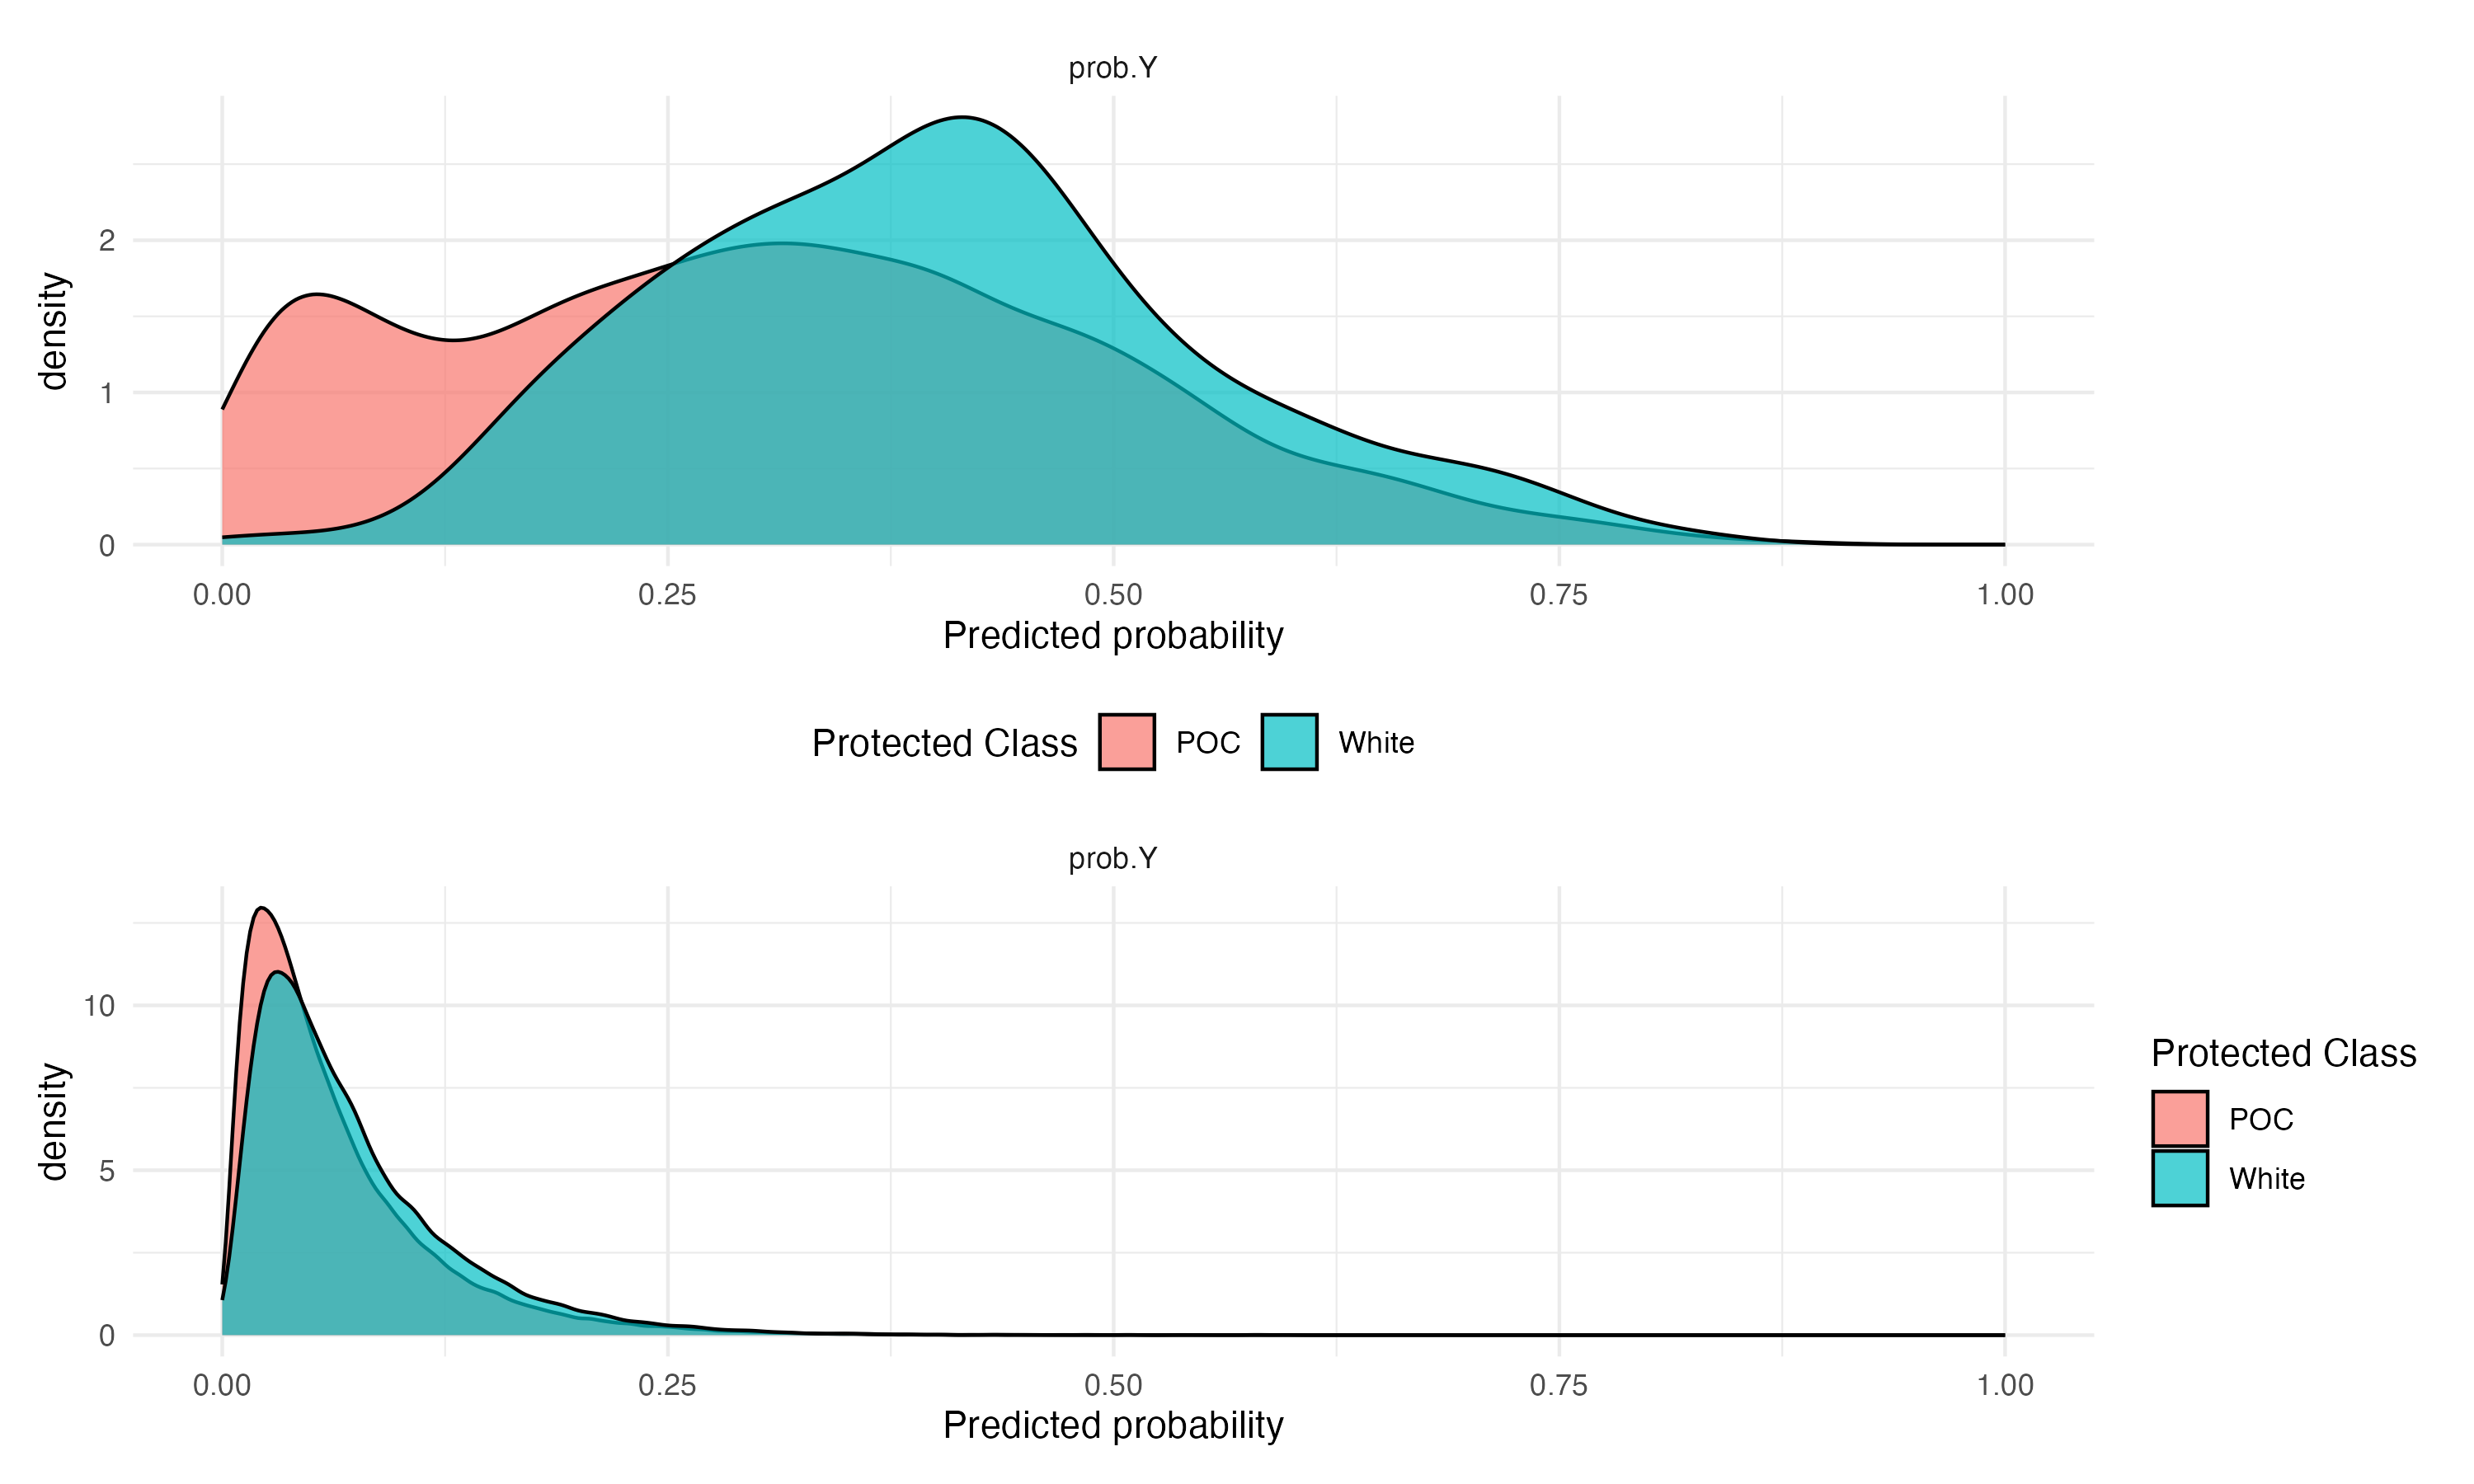
\includegraphics[width=0.7\textwidth]{../figures/sqf_case_study_plot7.png}
    \caption{Density of predicted probabilities both groups.}
    \label{fig:fairness_density}
\end{figure}
To train a random forest classifier on the 2023 data to predict the arrest of a person, we dichotomise the race attribute by grouping "Black" and "Hispanic" as people of colour ("PoC") and "White", "Asian", and "Other" as white ("White").
With many of the group fairness metrics implemented in mlr3fairness, we can measure the (group) fairness of our models.
As suspected after data description, we find that the random forest classifier is already fair. There are minor differences between groups, but exact equality cannot be expected. It is common to allow for a certain margin of error $\epsilon$ in practice.
Especially the error rates (fnr, fpr) are very similar between groups, thus Separation seems to be satisfied overall. Sufficiency metrics have larger differences, though they are still minor. mlr3fairness offers functions to easily visualise fairness. First, in \autoref{fig:fairness_density} we plot the density of risk scores output by the random forest for each group.
The risk score represents the probability of getting a positive prediction $P(\hat{Y} = 1)$, which is undesirable in the SQF context. White subjects tends to have higher predicted probabilities of being arrested, their mode lies around 0.15 while the mode of the PoC group is around 0.05. This means we have more low-risk PoC in the data. Next, from \autoref{fig:fairness_metrics_barplot} we can see that the positive predictive value (Sufficiency) has a relatively large difference between groups,
while the false positive rate is practically the same between groups (Separation). It comes to no surprise that equalised odds, which is based on error rates, is satisfied. Finally, the accuracy between groups is not as equal as the error rates, but the absolute difference is still smaller than 0.05, which is a common $\epsilon$ to choose.
Given that the classifier is fair from a group perspective, it does not make sense to experiment with any of the implemented fairness methods in mlr3. At most, we could try to address the disparities in sufficiency metrics, but the common methods in the package are designed to address concerns with independence or separation. \\
\begin{figure}
    \centering
    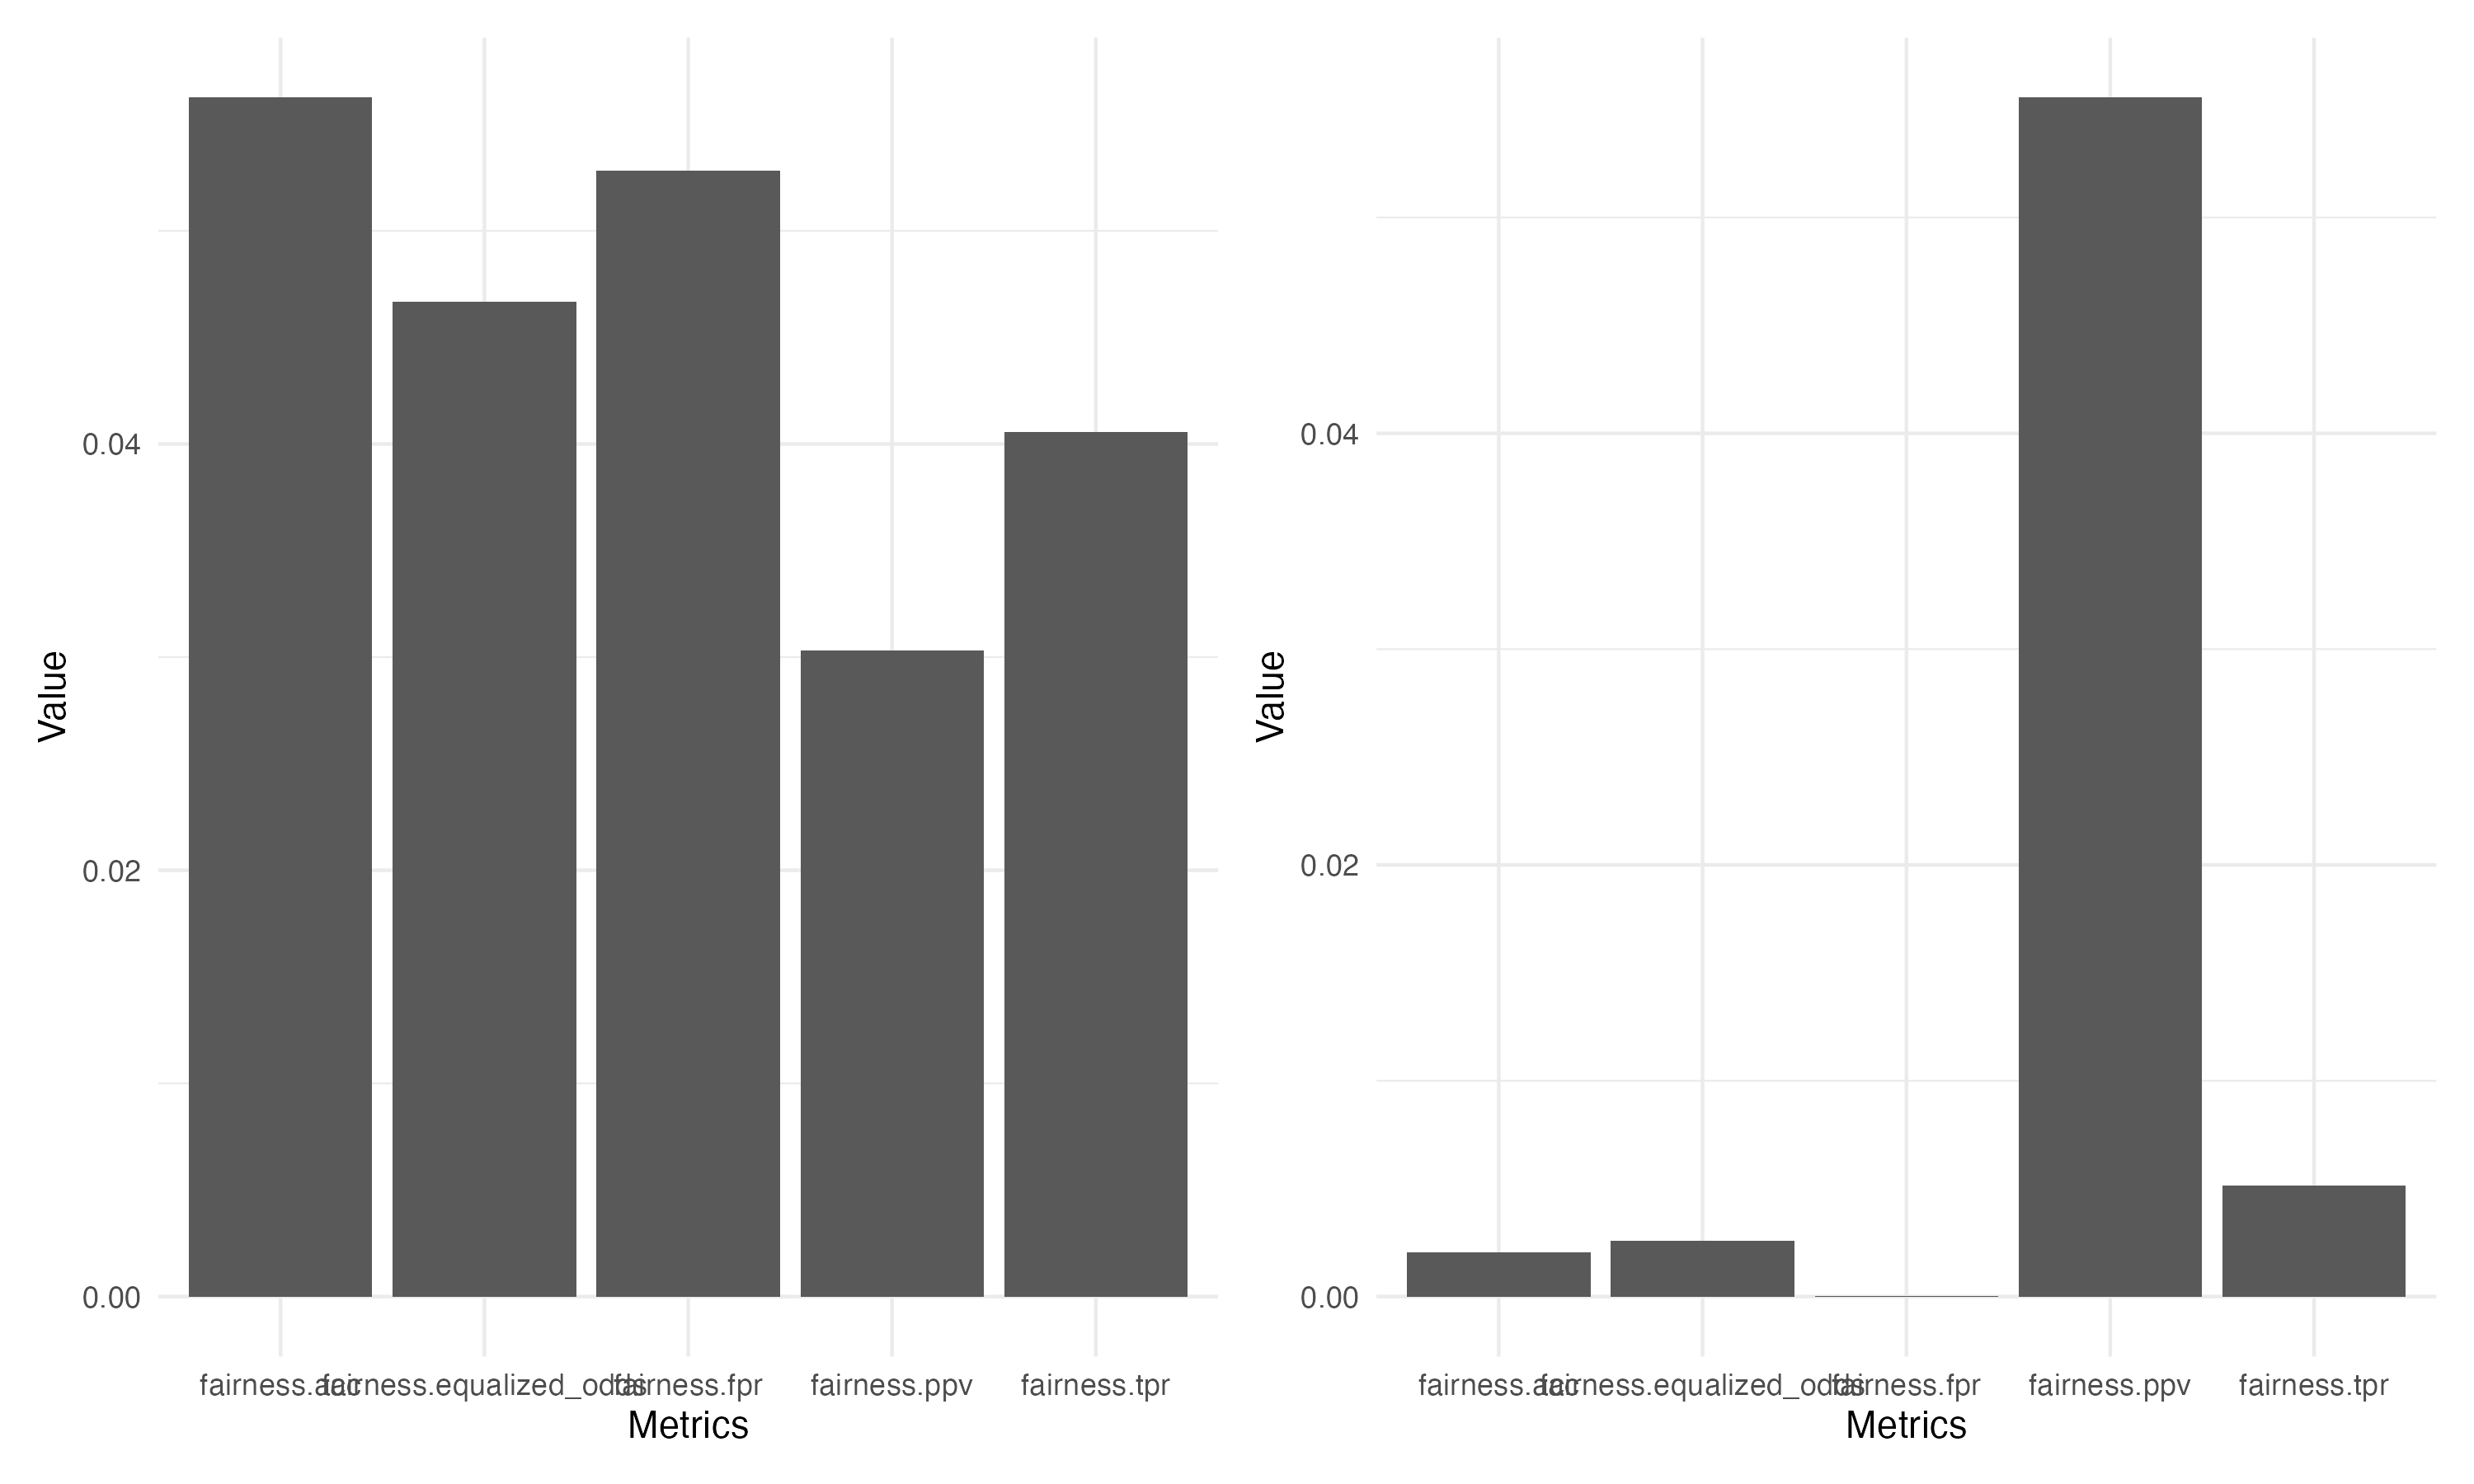
\includegraphics[width=0.7\textwidth]{../figures/sqf_case_study_plot8.png}
    \caption{Comparison of fairness metrics.}
    \label{fig:fairness_metrics_barplot}
\end{figure}

It is more interesting to compare the classifier trained on data that comes from the unconstitutional period 2004 to 2012. We decide for 2011 as it is the year with the most stops.
We carry out the same data cleaning steps for the 2011 data as before, starting with 685724 recorded stops and reducing this to 651567 clean observations. Note, these are more than 50 times more stops than in 2023.
The 2011 data has substantially more low-risk stops, only around 6\% of stops result in an arrest. This is a stark contrast to the 2023 data, where 31\% of stops result in an arrest.
The differences in arrestment rates between groups are slightly lower for 2011 and the highest arrestment rate remains to be for the white group. \autoref{fig:arrestment_rates_clean_data}
Due to the large proportion of low-risk stops in 2011 the predicted probabilities are generally low. The x-axis is cutoff at a probability of 0.1, otherwise it would be hard to see anything as the vast majority of probability mass lies in the small regions.
The measured racial disparities are interestingly not greater than in 2023. We see that for the classifier trained on 2011 stops, equalised odds has the greatest difference, but overall the differences in predictions rates across groups are very small. \\ 
Our fairness audit did not show any substantial disparities in fairness metrics. Does this mean the classifier is fair?
It is easy to come to such conclusions, especially if fairness is not the major concern of the practitioners but more of a nuisance criterion that should be fulfilled. However, to truly ensure a fair practice, it is crucial to look at the context in which the algorithm is embedded.

\begin{figure}
    \centering
    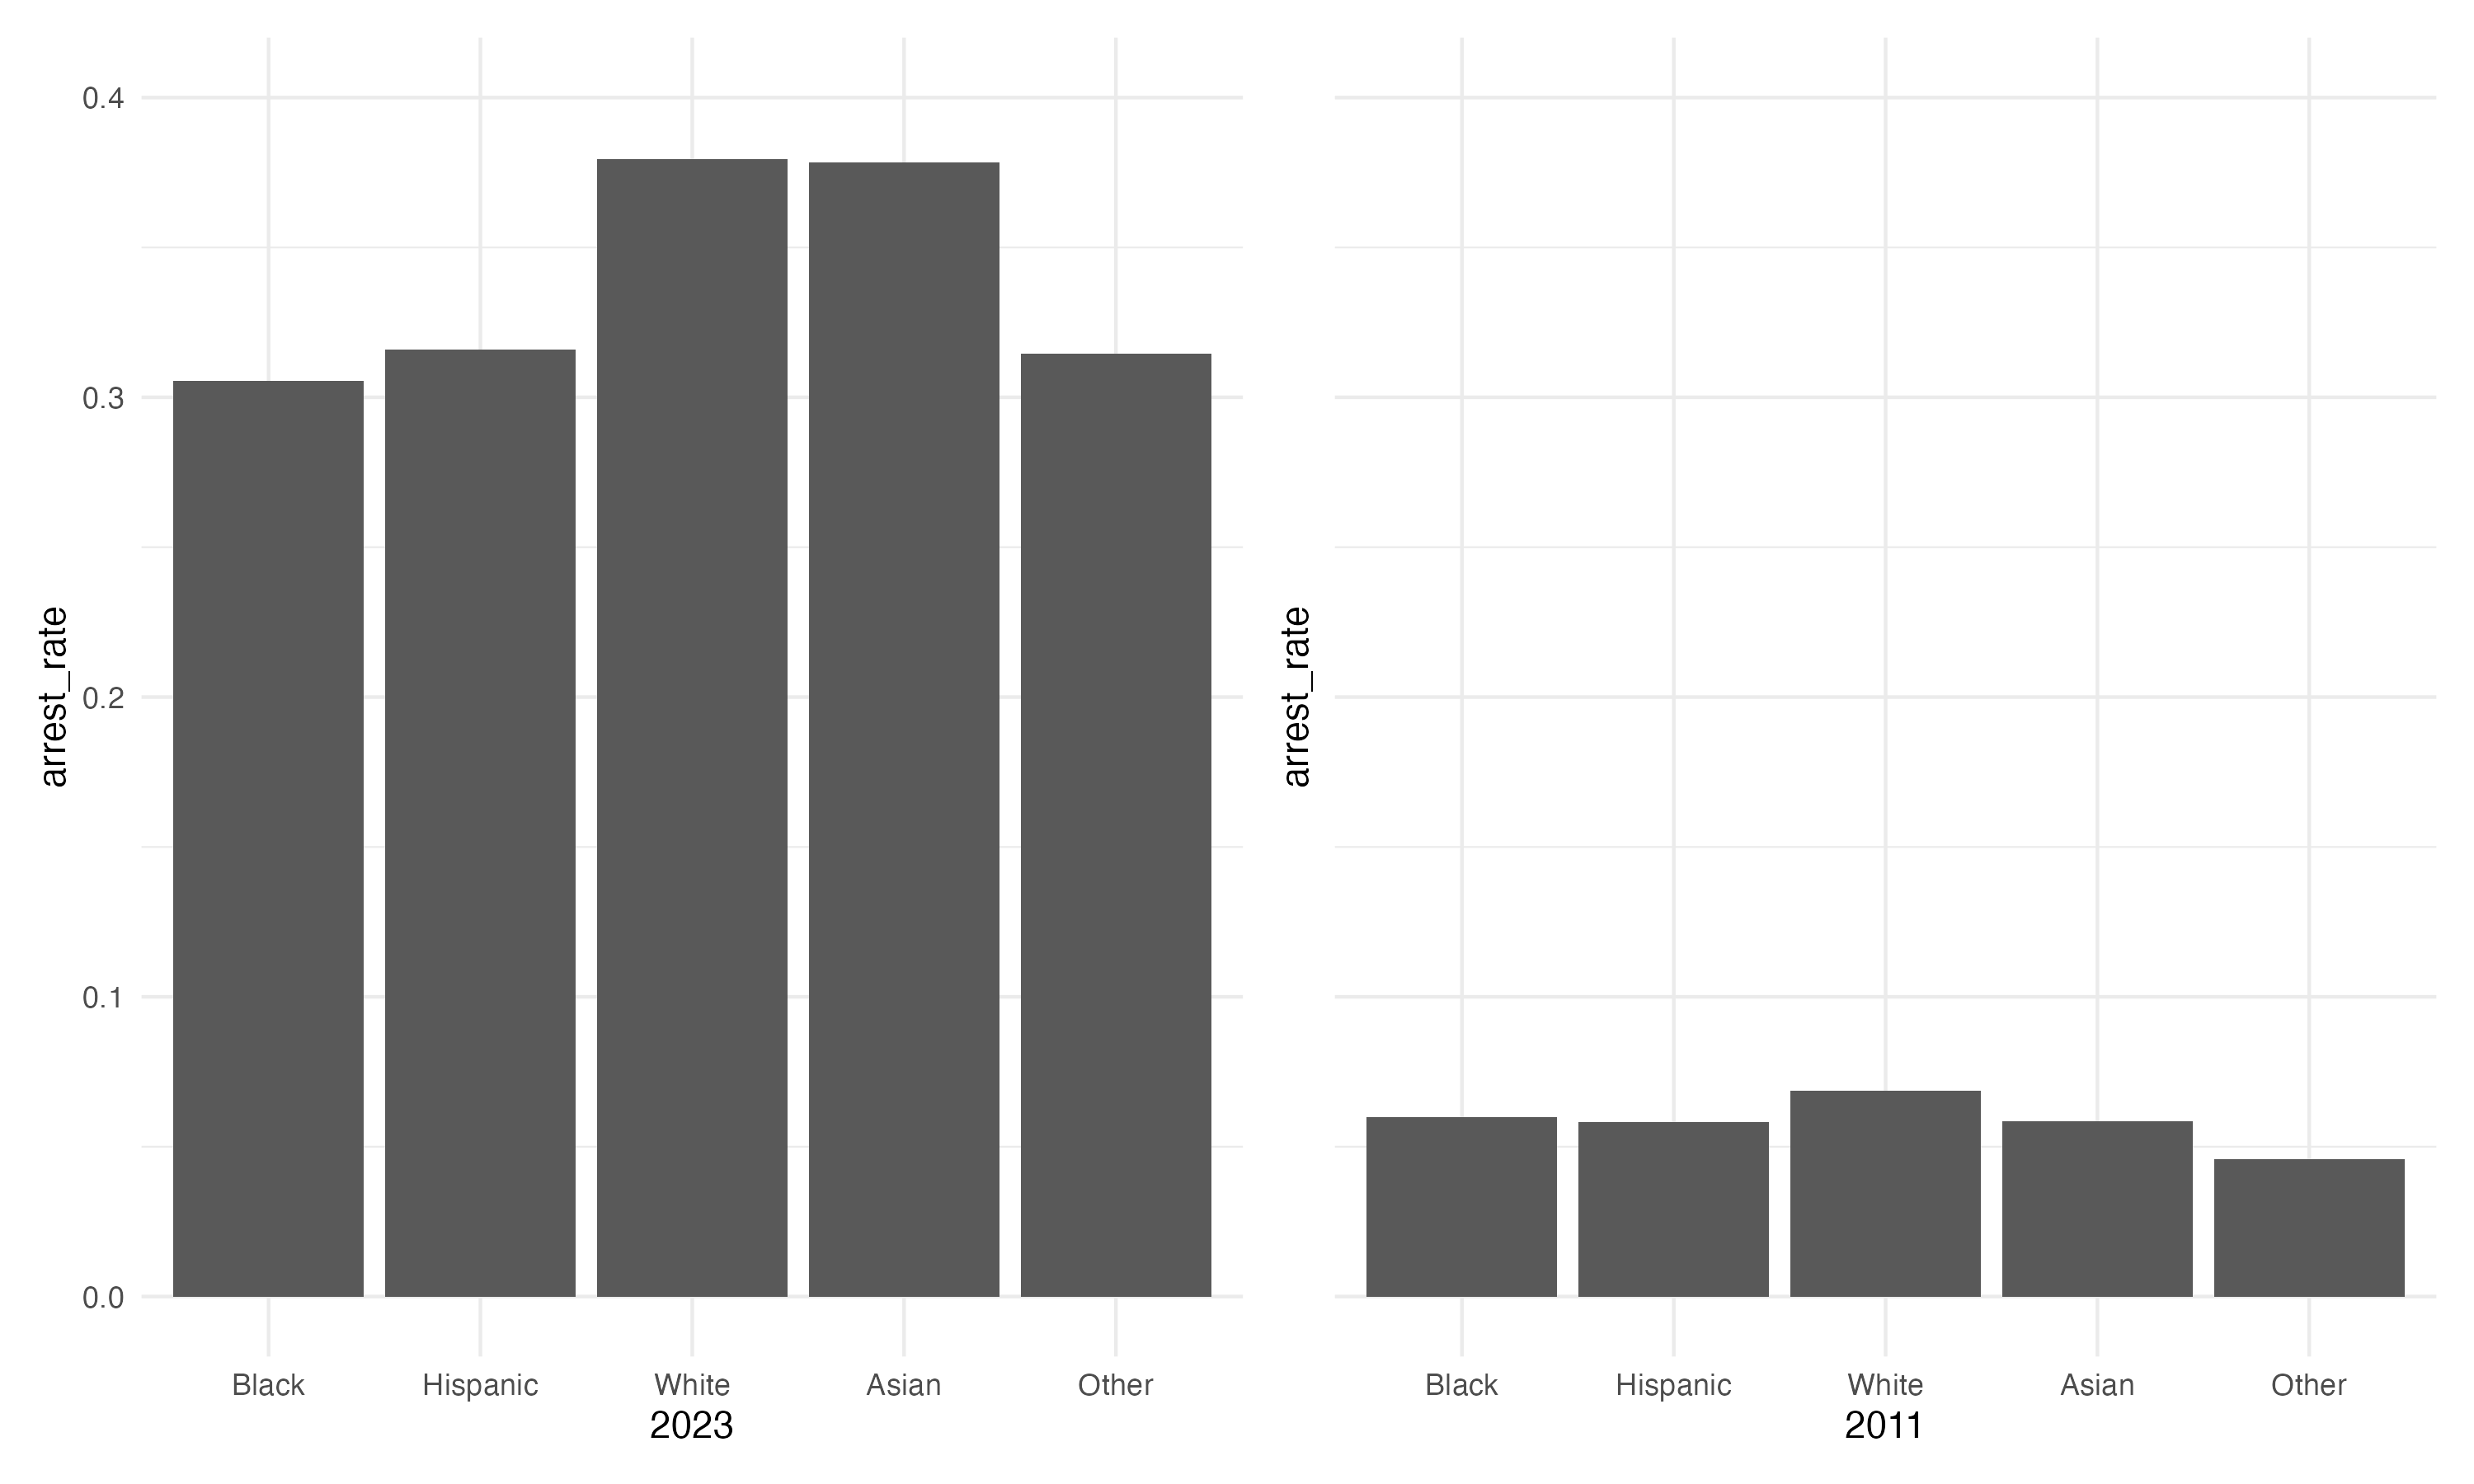
\includegraphics[width=0.7\textwidth]{../figures/sqf_case_study_plot10.png}
    \caption{Comparison of arrestment rates for 2023 (left) and 2011 (right).}
    \label{fig:arrestment_rates_clean_data}
\end{figure}

% \textbf{Fairness Experiment}
% - fairness metrics (table) for dichotomised race and for full race grouping in appendix.
% - fairness methods (inspired by the article)

% Reweighing: https://mlr3fairness.mlr-org.com/reference/mlr_pipeops_reweighing.html?utm_source=chatgpt.com#format
% Fair logistic regression: https://rdrr.io/cran/mlr3fairness/man/mlr_learners_classif.fairzlrm.html?utm_source=chatgpt.com
% EOd: https://mlr3fairness.mlr-org.com/reference/mlr_pipeops_equalized_odds.html?utm_source=chatgpt.com
% mlr3book: https://mlr3book.mlr-org.com/chapters/chapter14/algorithmic_fairness.html?utm_source=chatgpt.com#bias-and-fairness
% https://mlr3fairness.mlr-org.com/#debiasing-methods


% mlr3fairness currently has two preprocessing methods, one postprocessing method and several fairness adjusted models implemented. We decide to use a reweighing methods that works with assigning weights to the observations to equalise the distribution of $P(Y|PA)$.
% The inprocessing method is a fairness-adjusted logistic regression implemented in mlr3fairness inspired by Zafar et. al. This method optimises for statistical parity (independence). The postprocessing method we choose aims for equalised odds and it works by randomly flipping a subset of predictions with pre-computed probabilities in order to satisfy equalised odds constraints.
\subsubsection*{Bias and the feedback loop}
\begin{figure}
    \centering
    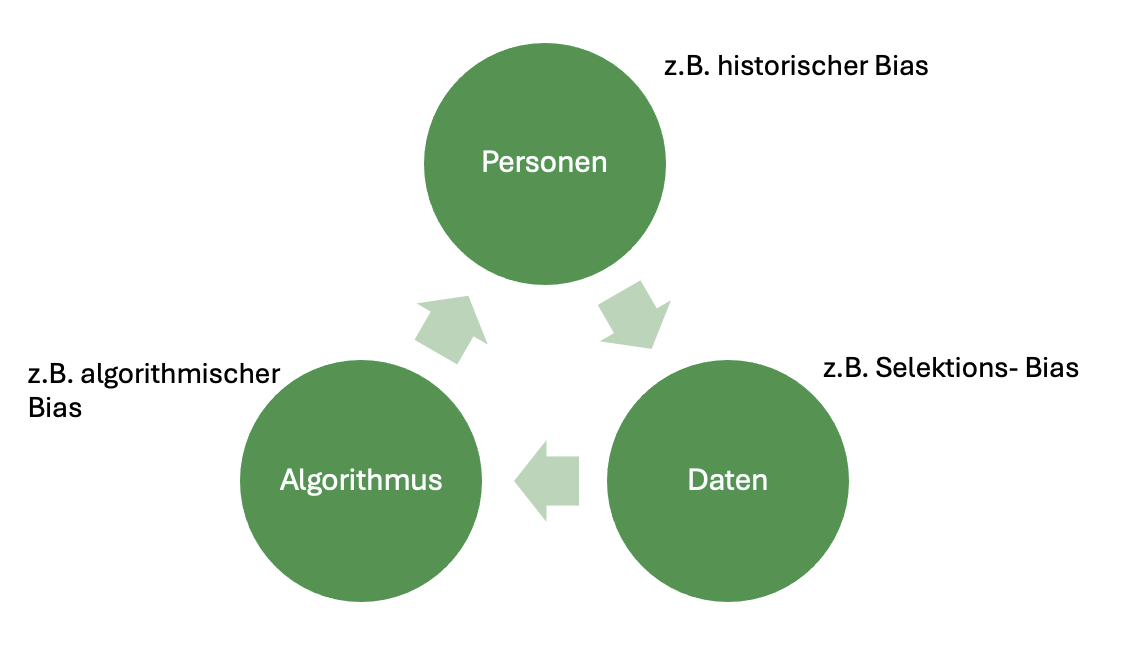
\includegraphics[width=0.7\textwidth]{../figures/bias_loop.png}
    \caption{The bias loop.}
    \label{fig:bias_loop}
\end{figure}

Usually fairness is a concern in the first place, because the algorithm should be implemented as an ADM to assist decision-making in some way. As such it could influence if someone gets admitted to college, gets a loan or is released from prison. The algorithm does not exist in isolation, but is embedded in a loop with data and the user.
We make the circumstances of a decision measurable by collecting data. The algorithm learns from this data to make an optimal prediction, on which the decision-makers base their judgement on ()\autoref{fig:bias_loop}). At each step of this loop, bias can be introduced in the process and, more dangerous, be amplified as the algorithm influences decision-making on a large scale.
This means that every fairness project comes with the task to understand where the data comes from and how exactly the algorithm will be deployed in practice. Let us therefore take a step back and look at the context of the SQF data.

% The data introduced three main challenges: selection bias; missing data; class imbalance.



% borough specific graphics?

% - number of stops conducted but with background information who governed at that time (see Obsidian)
% - transparent explanation of feature selection (similar to Data Transparanecy paper)
% - distribution of race in SQF data vs NYC
% - grouping to black, white, black hispanic, white hispanic, others --> arrestment rates in these groups


